% -------------------------------------------------------
\section{ARIMA with Structural Break Dummies}
% -------------------------------------------------------

Adding the two step dummies to the ARIMA specification yields an LM with 
ARIMA$(2,0,3)(0,0,1)_{12}$ errors. The break dummy for December 2012 carries 
a coefficient of $-0.568$ (s.e.\ $0.236$), consistent with the deflationary 
period following the sovereign debt crisis, while the August 2021 dummy 
carries a coefficient of $0.681$ (s.e.\ $0.264$), capturing the upward shift 
in the inflation mean during the post-COVID surge. In-sample fit improves 
noticeably, with AICc falling from $213.43$ to $204.04$.

Out-of-sample, however, the model is marginally worse than the plain ARIMA, 
with RMSE rising to $0.572$ and MAE to $0.509$. The Ljung-Box test continues 
to reject white noise residuals ($Q = 42.28$, $p = 0.001$). This divergence 
is consistent with a well-known limitation of structural break dummies in 
forecasting: once the break has occurred and the new regime has settled, the 
dummies provide little additional signal for future values 
\parencite{clements2002}. The plain ARIMA benchmark therefore remains the 
more competitive model out-of-sample.


% -------------------------------------------------------
\section{Dynamic Regression Models}
% -------------------------------------------------------

Three dynamic regression models are estimated, progressing from simple to 
data-driven. All three include the two structural break dummies and use 
first-differenced unemployment as regressors where applicable.

\textbf{Model A} regresses Danish inflation on lags 0 to 3 of first-differenced 
Danish unemployment. The unemployment coefficients are all positive and small, 
with none exceeding $0.055$, and the model yields an out-of-sample RMSE of 
$0.613$ and MAE of $0.544$, both worse than the ARIMA benchmark. There is no 
evidence that domestic labour market conditions carry useful forecasting 
information for Danish inflation in this sample.

\textbf{Model B} extends Model A by additionally including lags 0 to 3 of EU27 
inflation. Despite the strong in-sample co-movement between Danish and EU27 
inflation, out-of-sample performance deteriorates sharply to RMSE $1.208$ and 
MAE $1.039$, more than double the benchmark. The combination of unemployment 
and EU27 inflation appears to amplify forecast errors rather than reduce them.

\textbf{Model C} implements the GETS-selected specification, regressing Danish 
inflation on EU27 inflation at lags 0, 1, and 6, with both structural break 
dummies retained for economic reasons. AICc minimisation selects an LM with 
ARIMA$(1,0,2)(1,0,2)_{12}$ errors. The estimated coefficients are reported in 
Table~\ref{tab:modelC_coef}.

\begin{table}[H]
\centering
\caption{Model C coefficient estimates}
\begin{tabular}{lcc}
\hline
Parameter & Estimate & Std. Error \\
\hline
AR(1)            &  0.962 & 0.019 \\
MA(1)            &  0.060 & 0.063 \\
MA(2)            & -0.211 & 0.062 \\
SAR(1)           &  0.791 & 0.101 \\
SMA(1)           & -1.540 & 0.106 \\
SMA(2)           &  0.694 & 0.078 \\
break\_2013      & -0.427 & 0.162 \\
break\_2021      &  0.592 & 0.207 \\
EU27 infl.\ $t$  &  0.696 & 0.059 \\
EU27 infl.\ $t-1$ &  0.132 & 0.059 \\
EU27 infl.\ $t-6$ & -0.086 & 0.055 \\
\hline
\multicolumn{3}{l}{$\hat{\sigma}^2 = 0.073$, AICc $= 94.78$, BIC $= 137.23$} \\
\hline
\end{tabular}
\label{tab:modelC_coef}
\end{table}

In-sample fit improves substantially, with AICc falling to $94.78$ and 
residual variance dropping to $0.073$. The contemporaneous EU27 inflation 
coefficient of $0.696$ is large and precisely estimated, consistent with the 
tight co-movement observed in the data. The Ljung-Box test, however, continues 
to indicate residual serial correlation ($Q = 34.01$, $p = 0.013$), suggesting 
that the extreme observations during the 2021 to 2023 inflation surge are not 
fully absorbed by the standard ARIMA error structure.

Out-of-sample, Model C yields RMSE of $0.767$ and MAE of $0.637$, worse than 
the ARIMA benchmark despite its substantially better in-sample fit. The EU27 
inflation signal, while highly informative in-sample, appears to amplify 
forecast errors in the 2024 to 2026 test window, a period in which both Danish 
and EU27 inflation were rapidly normalising from post-surge levels 
\parencite{clements2002}.


\section{gammel konkludsion}

Table~\ref{tab:model_comparison} summarises out-of-sample forecast accuracy 
across all five models over the 24-month test period.

\begin{table}[H]
\centering
\caption{Out-of-sample forecast accuracy (test period: April 2024 to March 2026)}
\begin{tabular}{lcc}
\hline
Model & RMSE & MAE \\
\hline
ARIMA baseline                           & 0.567 & 0.471 \\
ARIMA with break dummies                 & 0.572 & 0.509 \\
Model A (DK unemployment)                & 0.613 & 0.544 \\
Model C (GETS: EU27 inflation)           & 0.767 & 0.637 \\
Model B (DK unemployment + EU27 inflation) & 1.208 & 1.039 \\
\hline
\end{tabular}
\label{tab:model_comparison}
\end{table}

The univariate ARIMA benchmark produces the lowest RMSE and MAE across all 
models. Every multivariate specification performs worse out-of-sample, and the 
ranking is monotone: adding more predictors consistently worsens forecast 
accuracy. Model B is the worst performer by a wide margin, with RMSE more than 
double the benchmark. This is consistent with a well-documented finding in the 
inflation forecasting literature that multivariate models often fail to 
outperform univariate benchmarks out-of-sample, particularly over short horizons 
and in periods of regime change \parencite{stock_watson_2008}.


gammel arima:

% -------------------------------------------------------
\section{ARIMA Benchmark}
% -------------------------------------------------------

\subsection{Full-Sample ARIMA}




Nye resultater Best model: ARIMA(4,0,5)(0,0,1)[12] with zero mean  


AICc minimisation over a grid of candidate specifications selects an ARIMA$(4,0,1)(0,0,1)_{12}$ model with a constant. The estimated coefficients  are reported in Table~\ref{tab:arima_coef}. The four AR terms reflect the  persistence in Danish inflation, while the seasonal MA term confirms the residual seasonal pattern identified in the inspection stage. \textcolor{red}{Det passer vel ik, var det ik kun for unemployment vi gjorde det.} 



\begin{table}[H]
\centering
\caption{ARIMA$(4,0,1)(0,0,1)_{12}$ coefficient estimates}
\begin{tabular}{lcc}
\hline
Parameter & Estimate & Std. Error \\
\hline
AR(1)    &  1.866 & 0.114 \\
AR(2)    & -1.089 & 0.171 \\
AR(3)    &  0.411 & 0.124 \\
AR(4)    & -0.197 & 0.063 \\
MA(1)    & -0.641 & 0.104 \\
SMA(1)   & -0.581 & 0.054 \\
Constant &  0.017 & 0.003 \\
\hline
\multicolumn{3}{l}{$\hat{\sigma}^2 = 0.118$, AICc $= 213.43$, BIC $= 241.98$} \\
\hline
\end{tabular}
\label{tab:arima_coef}
\end{table}

The Ljung-Box test at lag 24 rejects serially uncorrelated residuals 
($Q = 38.35$, $p = 0.003$), indicating that the model does not fully capture 
all serial dependence in the training data. Figure~\ref{fig:06_arima_baseline} 
shows the 24-month out-of-sample forecast against actual Danish inflation. 
The model tracks the general level of inflation reasonably well, with actual 
values largely remaining within the 80 percent confidence band, though forecast 
intervals widen substantially over the horizon. Out-of-sample forecast accuracy 
yields an RMSE of 0.567 and an MAE of 0.471 percentage points, which serve as 
the benchmark for all subsequent models.

\begin{figure}[H]
\centering
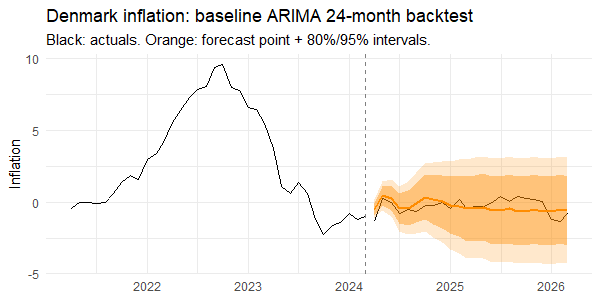
\includegraphics[width=0.5\linewidth]{billeder/06_Arima_baseline.png}
\caption{ARIMA baseline: forecast vs.\ actual Danish inflation}
\label{fig:06_arima_baseline}
\end{figure}



% Gammel qlr test:


\subsubsection{Structural break test (QLR)}

To test for structural instability in Danish inflation, we apply the Quandt Likelihood Ratio (QLR) test. The test searches over candidate break dates within the central 85 percent of the sample and identifies the date with the highest F-statistic. The sup-F statistic of 73.03 is highly significant ($p = 0.000$), leading us to reject the null hypothesis of parameter stability.

\begin{figure}[H]
    \centering
    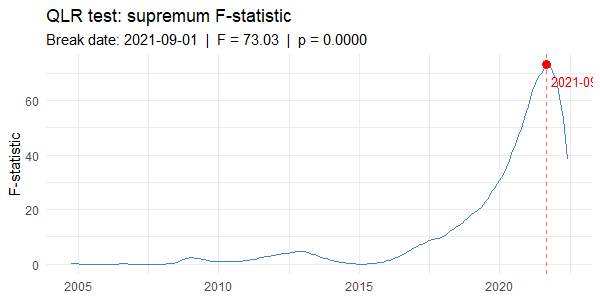
\includegraphics[width=0.5\linewidth]{billeder/05_QLR_struc_break_test.png}
    \caption{Structural break test}
    \label{fig:05_struc_break_test}
\end{figure}

We complement the QLR test with a Bai-Perron multiple breakpoint procedure. The BIC-optimal partition identifies two structural breaks: December 2012 and August 2021. These breaks coincide with periods of substantial macroeconomic instability: the low-inflation environment following the European sovereign debt crisis and the post-COVID inflation surge driven by supply-chain disruptions and energy price shocks.

The results suggest that Danish inflation is not governed by a single stable regime over the full sample. We therefore include post-break dummy variables in selected forecasting models to account for these regime shifts in a parsimonious and interpretable way. As a robustness check, we also use IIS/SIS within the GETS framework to detect additional outliers and step shifts. However, IIS/SIS is not used as the main break-handling strategy, since its flexibility may introduce many intervention dummies and increase the risk of overfitting. 

gammel gets sektion:


% The GUM included a constant, AR lags 1 to 6 of Danish inflation,
% contemporaneous and six lags of first-differenced Danish unemployment
% ($\Delta u^{\text{DK}}_{t-k}$, $k = 0,\ldots,6$), contemporaneous and six
% lags of first-differenced EU27 inflation ($\Delta \pi^{\text{EU}}_{t-k}$,
% $k = 0,\ldots,6$), and a bounded surge dummy equal to one from April 2021 to
% July 2023 and zero otherwise. The surge dummy was included as a selectable
% regressor rather than a fixed term, so GETS could freely eliminate it if the
% data did not support it. The model was estimated on 267 observations at the
% ten percent significance level with White-robust standard errors.

% After GETS reduction, all seven lags of first-differenced Danish unemployment
% were eliminated as statistically insignificant, consistent with the Granger
% causality results in Section~\ref{sec:granger}. The surge dummy was likewise
% eliminated ($p = 0.292$ in the GUM), indicating that the EU27 inflation
% channel already absorbs the co-movement during the 2021--2023 surge without
% requiring a separate level correction. The retained specification is
% \begin{equation}
% \pi_t = 0.074 + 0.973\,\pi_{t-1} + 0.068\,\pi_{t-3} - 0.082\,\pi_{t-6}
%       + 0.716\,\Delta\pi^{\text{EU}}_{t}
%       + \hat{\varepsilon}_t
% \label{eq:gets_specific}
% \end{equation}

% \textcolor{red}{der var de her og de her der overlevede vores get, og forklar - drop ligning}

% \begin{table}[h]
% \centering
% \caption{Model 4 coefficient estimates}
% \small{
% \begin{tabular*}{\textwidth}{@{\extracolsep{\fill}}lccccc}
% \hline \hline
% \rule{0pt}{12pt}\textbf{Parameter} & Const & AR(1) & AR(3) & AR(6) &
% $\Delta \pi^{\text{EZ}}_{t}$ \\[4pt]
% \hline
% \rule{0pt}{12pt}\textbf{Estimate} & $0.074$ & $0.973$ & $0.068$ & $-0.082$ &
% $0.716$ \\[4pt]
% \rule{0pt}{12pt}\textbf{Std. err} & $(0.035)$ & $(0.059)$ & $(0.073)$ &
% $(0.042)$ & $(0.086)$ \\[4pt]
% \hline \hline
% \multicolumn{6}{l}{\rule{0pt}{12pt}\footnotesize $\hat{\sigma}^2 = 0.113$,\;
% AICc $=180.8$,\; BIC $=198.7$.}
% \end{tabular*}
% }
% \label{tab:model4_coef}
% \end{table}

% \noindent with $R^2 = 0.971$ and $\hat{\sigma} = 0.336$.
% The contemporaneous EU27 inflation change is highly significant
% ($t = 8.28$, $p < 0.001$), confirming the ERM\,II spillover channel. The AR(3) term is retained despite not individually clearing the ten percent threshold ($p = 0.354$), a known property of the GETS path-search: a regressor survives if removing it in any explored elimination path worsens residual diagnostics or destabilises other retained coefficients. Ljung-Box AR(7) yields $p = 0.678$, so residual serial correlation is not detected. The ARCH(1) test yields $p = 0.035$, a marginal rejection of homoskedasticity; White-robust standard errors are used throughout so inference remains valid.

% Out-of-sample, the model attains an RMSE of $0.546$ and MAE of $0.491$ over
% the 24-month test period, with a mean error of $0.238$, indicating a small
% systematic over-prediction. This is essentially identical to the pre-surge
% ARIMA benchmark ($\text{RMSE} = 0.54$), confirming that the EU27 spillover
% channel is informative in-sample but contributes negligible incremental
% forecast content beyond what the univariate benchmark already captures. The
% elimination of both unemployment and the surge dummy by GETS provides a direct
% answer to the Phillips curve question: neither domestic labour market
% conditions nor a structural break correction improve upon the inflation
% dynamics already explained by autoregressive lags and contemporaneous EU27
% inflation.
